% !TEX encoding = UTF-8
% !TEX TS-program = pdflatex
% !TEX root = ../tesi.tex

%**************************************************************
\chapter{Svolgimento del progetto}
\label{cap:ilprogetto}
%**************************************************************

% \intro{Breve introduzione al capitolo}

%**************************************************************
\section{Analisi e pianificazione}

\subsection{Analisi}
Il mio stage è iniziato quando ormai l'analisi era finita, quindi non ho avuto nessun contatto con il proponente. Tuttavia sono stato messo subito al corrente dei
requisiti individuati e sono stati inseriti negli obiettivi del progetto di stage, quindi già esplicati nel capitolo precedente. Essendo un refactoring di un applicazione
già esistente parte dei requisiti erano già stati stabiliti, quindi elencherò i principali cambiamenti richiesti. Utilizzerò come notazione R+(F|Q|V)+X+(D|O), dove:

\begin{itemize}
  \item R: requisito;
  \item F: funzionale;
  \item Q: qualitativo;
  \item V: di vincolo;
  \item X: numero progressivo;
  \item D: desiderabile;
  \item O: obbligatorio;
  \item Z: opzionale.
\end{itemize}

Alcuni dei requisiti più importanti individuati sono riportati nella tabella \autoref{tab:requisiti}, con codice e relativa descrizione:

\renewcommand{\arraystretch}{2}
\begin{longtable}{|p{4cm}|p{10cm}|}%
  \caption{Tabella del tracciamento dei requisti funzionali} 
  \label{tab:requisiti} \\
  
    \hline
    \textbf{Requisito} & \textbf{Descrizione} \\
    \hline
    \endhead
    RF1O     & L'interfaccia permette di fare il login nel sistema gestionale di UCIS \\ \hline
    RQ2O     & L'applicazione riconosce se è già stato effettuato un login e utilizza i dati salvati per effettuarlo \\ \hline
    RQ3O     & L'applicazione deve funzionare offline se la persona è già autenticata \\ \hline
    RV5O     & I dati dell'account non vanno salvati nella memoria, ma nel sistema Android \\ \hline
    RF8O     & L'interfaccia permette di creare attività \\ \hline
    RF9O     & L'interfaccia permette di visualizzare un'attività \\ \hline
    RF10O     & L'interfaccia permette di avviare la registrazione di un'attività \\ \hline
    RV18O     & L'applicazione deve essere scritta con uno strumento che permetta lo stesso codice per tutte le piattaforme \\ \hline
\end{longtable}%

%**************************************************************
\subsection{Pianificazione}

Come specificato dal requisito RV18O si era alla ricerca di un framework crossplatform. Di seguito alcune delle tecnologie che abbiamo analizzato e alcuni dei motivi per
cui non sono stati scelti.

\subsubsection{Cordova e PhoneGap}

\begin{figure}[h]
	\begin{center}
		
\includegraphics[height=2.5cm]{cordova}
		\caption{Logo di Cordova}
	\end{center}
\end{figure}

La prima tecnologia con cui sono stato a contatto è stato il framework Cordova. Il software è stato acquisito da Adobe nel 2011 mantenendolo \gls{open source} e
rilasciandolo nel 2013 con il nome di Apache Cordova. Stiamo parlando di un framework che permette attraverso alcuni tools di creare applicazioni utilizzando CSS3, HTML5 e
Javascript, evitando allo sviluppatore di affidarsi alle API specifiche del sistema operativo. Il pregio di questa tecnologia è il fatto che la stessa
applicazione non dovrà essere scritta in Java per Android, in XCode o Swift per iOS, ma avrà un codice unico che sarà adattato per i singoli sistemi operativi. \\
Tutto ciò funziona tramite le WebView native. Le WebView sono delle componenti delle applicazioni utilizzate per visualizzare contenuti web. Queste sono
sviluppate dai sistemi operativi e non fanno altro che renderizzare ciò che è stato scritto con linguaggio HTML5, CSS3, Javascript. Per facilitarne la
comprensione si possono immaginare come delle pagine web visualizzate all'interno di un browser, senza gli elementi tipici di esso (come la barra dell'URL,
delle tab o le opzioni). \\
Le applicazioni sviluppate in questo modo si possono considerare sia in parte \gls{web-based}, sia in parte native perché utilizzano e hanno accesso a tutti i componenti
hardware della piattaforma sulla quale vengono eseguite. Ciò avviene tramite i plugin, che possono essere parte del framework, oppure, tramite API apposite,
scritti dallo sviluppatore stesso. Inoltre l'applicazione può essere impacchettata, installata o caricata negli store ufficiali come una qualunque altra nativa.
\\
La forza di Cordova e del fatto che sia open source, sta nel fatto che possiede una libreria vastissima di plugin utilizzabili che forniscono un controllo
totale sul dispositivo, come se si sviluppasse dal linguaggio nativo. Uno dei plugin che abbiamo immediatamente ricercato, è quello che si occupa del
tracciamento GPS continuo in \gls{background}. Siamo andati quindi a creare un primo prototipo di applicazione installando solamente quel plugin per semplice
test. Durante questo veloce procedimento abbiamo però riscontrato diversi problemi nell'installazione delle varie componenti o nella compatibilità con altre
librerie (come nel nostro caso con le \gls{SDK} di Android). L'impressione di questo software non è stata positiva, perché mi è sembrato vecchio
e poco mantenuto. Informandomi poi ho notato che le varie aziende, che lo utilizzavano come framework di sviluppo si stavano muovendo su altri software nuovi e
più aggiornati.\\
Menzione d'obbligo è da fare ad Adobe PhoneGap, nato come versione non \gls{open source} di Cordova, che fornisce a pagamento servizi molto interessanti, come ad
esempio la build in cloud dell'applicazione, eliminando i problemi derivati dall'ambiente di sviluppo sul quale si sta lavorando.

\subsubsection{Ionic e Capacitor}

\begin{figure}[h]
	\begin{center}
		
\includegraphics[height=2.5cm]{ionic}
		\caption{Logo di Ionic}
	\end{center}
\end{figure}

Ionic è un framework open-source rilasciato da Drifty Co. nel 2013. La prima versione di Ionic non era altro che un SDK che metteva a disposizione una
piattaforma AngularJS per lo sviluppo di applicazioni con Cordova. Le ultime versioni di Ionic hanno aggiunto nuove funzionalità, tra le
quali la possibilità di scegliere di sviluppare in Angular, React o Vue. Inoltre è stato rilasciato un software per la build e le API proprietario,
chiamato Capacitor, che racchiude al suo interno Cordova, aggiornandolo e adeguandolo alle nuove SDK dei vari Sistemi Operativi. Perciò derivando
da Apache Cordova, contiene tutte le sue funzionalità, e di conseguenza tutti i suoi pregi, ma anche alcuni dei suoi difetti. \\
Testando Ionic mi sono accorto di alcuni punti deboli delle applicazioni ibride. \\
In primo luogo le performance. Le applicazioni ibride hanno bisogno della WebView che non è altro che un altro processo di supporto per
renderizzare pagine web. Inoltre è un dato di fatto che le applicazioni web sono molto esose dal punto di vista delle risorse rispetto a un
applicazione scritta in linugaggio nativo per quel dato sistema operativo. In secondo luogo non si ha controllo totale sui plugin che
servono a interfacciarsi con il dispositivo. Le librerie native sono molto più ricche e specifiche, ma soprattutto non richiedono
l'intervento di software di terze parti, come Ionic e Capacitor, per funzionare. Questi problemi sono emersi subito, una volta installato
ionic e fatto una veloce build dell'applicazione ci siamo accorti della poca reattività su dispositivi datati e della difficoltà nel
personalizzare i plugin messi a disposizione. \\
Come mai \acrlong{asd} si è messa in gioco in questo campo? Da alcune ricerche è emerso che la maggior parte delle aziende che sviluppano
per mobile si stanno muovendo verso le applicazioni ibride. I motivi non sono difficili da comprendere. Il fatto che un unico codice può
essere eseguito su diversi dispositivi è sicuramente un fattore molto importante. Finora le aziende dovevano sviluppare applicazioni diverse
quindi moltiplicando il costo e le risorse. Supponendo di utilizzare solo linguaggi nativi, \acrlong{asd} avrebbe dovuto sviluppare almeno
due appplicazioni differenti, una per Android e una per iOS, riutilizzando pochissimo codice e impiegando almeno il doppio di risorse.
Sarebbero stati necessari almeno altri due sviluppatori e i tempi di fornitura sarebbero stati decisamente più lunghi. 

\begin{wrapfigure}{l}{0.45\textwidth}
  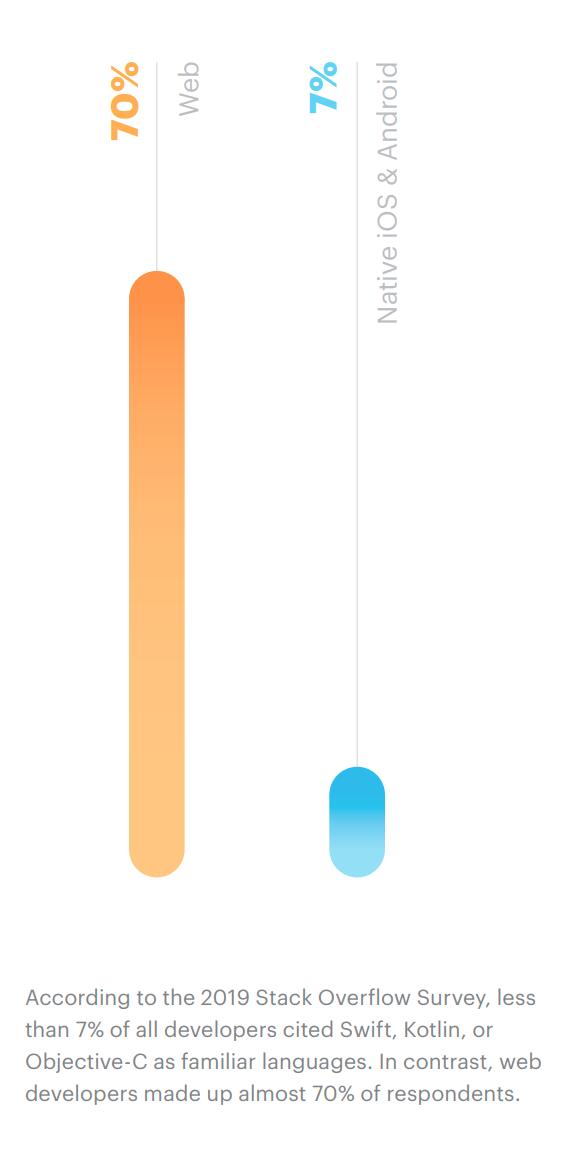
\includegraphics[width=0.9\linewidth]{sviluppatori} 
  \caption{Caption1}
  \label{fig:sviluppatori}
\end{wrapfigure}

Inoltre gli sviluppatori con esperienza in API native non sono molto comuni. Non sono rari invece sviluppatori web, dei quali fa parte anche il mio
tutor, come dimostra la figura \autoref{fig:sviluppatori}. \\
Da notare anche come il mondo si stia muovendo molto velocemente verso il web. Moltissime delle applicazioni tuttora si basano su tecnologie
che sono sviluppate per esso, come AWS di Amazon, Azure di Microsoft, Google Cloud e molti altri. Sviluppare in questo senso è
anche un investimento su un mondo che è aperto a opportunità continue e di conseguenza al futuro.

\subsubsection{Flutter}
Nonostante mi ritenessi soddisfatto dell'impressione di Ionic, ho preso in cosiderazione un'ultima alternativa, Flutter. Flutter è un
framework che si occupa della creazione di interfacce grafiche native per iOS, Android e desktop. Sviluppato da Google e rilasciato nel
2017, Flutter utilizza un linguaggio proprietario Dart, presentato come alternativa a Javascript. L'engine, sviluppata in \gls{C++}, si occupa di
renderizzare i widget, oggetti grafici scritti dallo sviluppatore, 